\documentclass[sigconf]{acmart}
\usepackage{booktabs} % For formal tables
\usepackage{graphicx}
\usepackage{CJKutf8}
\usepackage{multirow}

\begin{document}
\title{Persuasively Explainable Recommendation}

\author{Submission }


\begin{abstract}
In the e-commerce environment, it is a personalized service to recommend suitable products according to the shopping scene of the user. We hope to provide users with an explainable and persuasive recommendation reason when recommending products, that is, why they should recommend this product, and motivate online purchasers to make successful purchases through persuasive descriptions. In this contribution we present our system by combinning weak supervision frame with generate model.  We first select the persuasive sentences from corpus as the training data of our generate model through weak supervision. Then through our proposed model yield persuasive sentence. We conduct comprehensive experiments on real sets. Compared with state-of-the-art methods, our framework produces sentences with higher ROUGE and BLEU scores and more attractive and persuasive.

\end{abstract}

\keywords{persuasive, explainable,recommendation}


\maketitle

\section{INTRODUCTION}
%1.explainable recommendation: importance
%shall we restrict motivation in industry?
To provide accurate recommendation, state-of-the-art recommendation systems depend on complex machine learning models on heterogeneous data sources. 
These models function as black boxes, which is a major obstacle to improving user experience and increasing user stickness. 
Aiming to overcome this obstacle, there is growing interest in developing \textit{explainable recommendation} systems to provide intuitive explanations of the recommendation results. 
In particular, recently many E-commerce sites such as Alibaba and Amazon invest heavily in providing automated recommendation explanations~\cite{}, motivated by the success of promoting sales using manually-written recommendation reasons. 

%explainable recommendation: persuasiveness and effectiveness
Explanations can benefit recommender systems on a number of aspects. As defined in~\cite{Tintarev2011Designing}, there are seven categories of recommendation explanations, working respectively to improve the degree of system transparency, scrutability, trust, effectiveness, persuasiveness, efficiency and satisfaction. 
From the viewpoint of E-commerce sites, \textit{persuasiveness} and \textit{effectiveness} are the most desirable aspects.


\textit{Persuasiveness} is the ability to convince users to buy the recommended items. 
An ideal example of \textit{persuasiveness explanation} for each item is to compose creatively a catchy and appealing sentence that is enjoyable to read.
As it directly associates with conversion rates, an industry-level explainable recommendation system must focus primarily on generating persuasive explanations.  

\textit{Effectiveness} is the power to help users make better purchase decisions.
Ultimately, custom need is the driver of purchase decision. 
A practical and efficient way to describe customer needs is to categorize them into different \textit{scenes}, under which customers purchase products or services to function.
An example scene takes place on the beach in summer, which prompts swimsuit purchases. 
With the help of a taxonomy of scenes, \textit{effective explanation} describes the utility of each item in a manner of how the item suits user preference under the user's intended scene.
This type of effective explanation can facilitate user decision process. It will reduce E-commerce product return rate and reduce enterprise cost.
In addition, effectiveness and persuasiveness are highly correlated.  As found in many surveys in advertising, information can have a powerful impact on liking~\cite{}. Infusing explanation with information on how the user can utilize an item strengthens the explainability power of the recommendation system.  

\begin{figure}\label{fig:example}
\caption{An illustrative example which is the real output of our system.}
\end{figure}

However, existing explainable recommendation systems mostly concentrate on aspects other than persuasiveness and effectiveness.  The majority of previous work aims to improve system transparency by devising interpretable models (i.e. factor models~\cite{Zhang et al. [2014a] and Zhang [2015]}) which lead to feature level explanation. Explanations have been offered as charts~\cite{Hou et al. [2018] u}, word clouds~\cite{Wu and Ester [2015] }, highlighted regions of the product images (Chen et al. [2018c), or merged phrases in a textual template~\cite{Zhang et al. }. 
It is widely accepted that computers which convey personality are more persuasive~\cite{Yoo2011Creating}. The lack of free text makes an explainable recommendation system less humanly, thus weakens its power to be persuasive. 

We notice that there is an emerging trend in studying persuasive systems, including  a recent work on transforming given specification of an item to persuasive descriptions~\cite{}. Although they have been been useful in E-commerce sites to attract consumers, they do not satisfy the personalized demands in recommendation systems. They are not able to tailor both persuasive and informative explanations that are relevant to specific user needs, which is precisely the goal of our work.

In this paper we propose an explainable recommendation system. Given a user's historical behavior, an item's profile, and an in-house scene taxonomy, we provide a  \textbf{persuasive} and \textbf{effective} recommendation reason. The explanation is post-hoc, as it is not generated from the recommendation model. We allow the flexibility of adopting any recommendation model, which is not discussed throughout the paper. Our explanations describe several key features extracted from the item's profile and elaborate that these features are charming under the user's intended scene. As shown in Figure.~\ref{}, the explanation "the one-piece's very low neckline gives it extra sex appeal on the beach" relates the item feature "low neckline" to the intended scene "beach" in a very persuasive style.  

To develop such a system, we face two challenges.  The first challenge arises from the insufficiency of training data. Deep sequence models have made remarkable success in generating readable texts in natural language. However, such success has been fueled by large-scale supervision. It is prohibitively expensive to label persuasive sentences due to the extremely subjective and diverse nature of persuasiveness. Persuasiveness is subjective, because different human judges have varying standards. It is costly to derive a gold standard that is approved by domain experts. Persuasiveness is diverse, because a persuasive sentence can be written in different styles.  It is impossible to list all variants of persuasive sentences.   
 
To address the first challenge, we turn to a framework with weak supervision. We program a set of rules with high coverage and low accuracy to generate training sets with noisy labels from external data source. To resolve the potentially conflicts among rules we xxx %work here?

The second challenge arises from the structure of dependency between between item features and scenes. Some features are universally perceived to be persuasive while some features are attractive only under specific scenes. For example, given a swimsuit, being ``high quality and cheap'' is good despite of any scene, , having. ``a low neckline'' under scene ``summer beach'' is good, under scene ``swim competition'' is bad. 
A naive solution is to construct training set for each scene.
However, the distribution of scenes is highly skew in user needs. For example, in the $30000$ scenes built in our in-house scene taxonomy, only $1\%$ are found to have xxxx. %need data.


To address the second challenge, we design to modules: a global module to encode universal persuasive patterns, a local module to encode scene-specific relations between persuasive ness and item features. Through a copying mechanism, we combine the global module and the local module.

Our contributions are three folds.
\begin{itemize}
\item In the application level, we present a novel explainable recommendation system. To the best of our knowledge, we are the first to provide persuasive and effective explanation by explaining how well the item suits user preferences under different scenes.
\item In the model level, we present a novel deep sequence model with a global module to learn universal persuasive patterns and a local module to learn scene-specific persuasive patterns.
\item In the evaluation level, we present a novel scheme as well as some easy-to-implement merits to evaluate the persuasiveness and effectiveness of our explanations. 
\end{itemize}


%paper structure
This paper is organized as follows. We briefly survey the related work in Sec.~\ref{sec:related}. In Sec.~\ref{sec:architecture}, we first introduce the architecture of our system and describe the weak supervision and our global-local-copy model. We present and analyze the experimental results on a real data set in Sec.~\ref{sec:experiment}. We conclude our work and suggest future directions in Sec.~\ref{sec:conclusion}.

\section{RELATED WORK}\label{sec:related}
\subsection{Explainable Recommendation}

In recent years, there have been many studies on natural language processing, including poetry creation \cite{Colton2012Full,Oliveira2015Tra,Ghazvininejad2016Generating,Yi2017Generating,Zhang2014Chinese,wang2016chinese},machine translation \cite{Kalchbrenner2016Neural,Zhou2016Deep,Wu2016Google}, and so on. A persuasive and explainable recommendation reason for the generation of goods, similar to the above two questions, is a sequence model. In fact, most ML research usually focuses on predictive tasks, but rarely provides explanations for them. However, many customers need to rely on the recommendation reasons provided by the system to be firm in their determination to purchase the item.

The traditional explainable recommendation method has content-based recommendation and collaborative filtering. \cite{vig2009tagsplanations,sigurbjornsson2008flickr} used tags as content features for recommendations and generate corresponding explanations. Collaborative filtering is divided into user-based collaborative filtering and item-based collaborative filtering. \cite{herlocker2000explaining, gedikli2014should,sarwar2001item} provided an explanation using the ratings of its neighbors or its similar items. In recent years, many models have attempted to use textual information to generate textual explanations for recommendations. One is to extract commodity features as an explanation, such as \cite{wu2015flame} used topic models to explain recommendations, \cite{zhang2017entity} found the related entities and gave conceptual explanation, the other is to generate complete sentences as an explanation, such as \cite{ozbal2013brainsup} generated textual explanation based on fixed templates, \cite{munigala2018persuaide} based on linguistic creativity to generate various forms of sentences. 

In this sense, Peake and Wang [2018] can be considered as a pointwise
post-hoc explanation model, while Singh and Anand [2018] can be
considered as a pair-wise or list-wise post-hoc explanation model.

natural language Costa et al. [2017] Li et al. [2017]
%not related to model
\subsection{Creative Text Generation}


\section{SYSTEM ARCHITECTURE}\label{sec:architecture}
We take the corpus of product as the input of our system, and produces a persuasive sentence with the scene description of the product. Fig.~\ref{fig:system-architecture} shows an overview of the proposed system architecture with two major steps: (1) Given the corpus of product,the first step is to select the persuasive sentences as the training data of our model, (2) identify the scene name, product name, cpv data \footnote{Cpv is a collection of values of the attributes of the product. Here, only the value of the product attributes is in the sentence it can be extracted.} from the selected sentence as the input of our model,then yield persuasive sentence. In this section, we first introduce the weak supervision method for selecting the persuasive sentences. We then present our global-local-copy model in detail.  

\begin{figure}
    \centering
    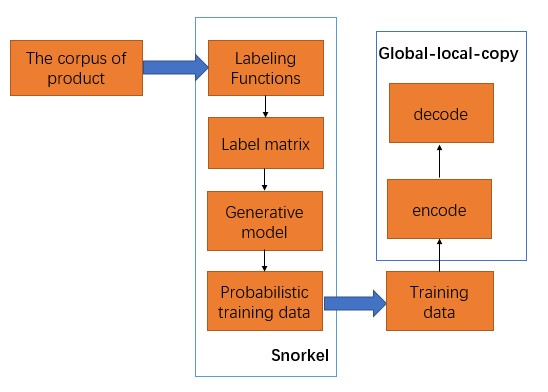
\includegraphics[width=8cm,height=5cm]{system-architecture.jpg}
\caption{System Architecture}\label{fig:system-architecture}
\end{figure}

\subsection{Resources Used}
% Data set
We use the list of product recommendation reasons as our dataset. The corpus are generated by high quality person.But the quality of the original dataset is far from ideal, there are many recommended reasons are even the original title of the product, so we need to filter the training data.

\subsection{Weak Supervision}
% Weak Supervision
Manual labeling is very time consuming, so we use the Snorkel \cite{ratner2017snorkel} weak supervision method to mark the data without the user to manually mark any training data. Rather than hand-labeling training data, users of Snorkel write labeling functions(LF), which allow them to express various weak supervision sources such as patterns, heuristics, external knowledge bases, and more. We wrote ten labeling functions based on the characteristics of persuasive sentences, is shown in Tab.~\ref{table:LF}. Among them, the labels of the first five functions are positive and the rest are negative.

\begin{table}
  \caption{Labeling Functions}
  \label{table:LF}
  \begin{tabular}{p{2.5cm}p{5cm}}
    \toprule
    Labeling Functions & Description\\
    \midrule
    %正类
    is\_neat & Sentence is neat\\
    has\_modal & Sentence has modal particle\\
    four\_word & Sentence contains a four-word structure \\
    dot\_word & The comma is followed by
        \begin{CJK*}{UTF8}{gbsn}
            "让/使/为/给"
        \end{CJK*}
        or verbs\\
    end\_exclamation & Sentence ends with an exclamation point\\
    %负类
    no\_adj\_and\_adv & Sentence has no adjectives and adverbs\\
    other\_words & Sentence contains characters other than Chinese, English, numbers, and specified symbols
        \begin{CJK*}{UTF8}{gbsn}
            (。,?!、;:).
        \end{CJK*}\\
    tree\_depths & the depth of the dependency tree is greater than 10\\
    clause\_num & the number of clauses is greater than 10\\
    token\_num & the number of word segments is greater than 10\\
  \bottomrule
\end{tabular}
\end{table}

Next, Snorkel automatically learns a generative model over the labeling functions,the output of Snorkel is a set of probabilistic labels. The statistics about the resulting label matrix is shown in Tab.~\ref{table:LabelMatrix}. \textbf{Coverage} is the fraction of candidates that the labeling function emits a non-zero label for. \textbf{Overlap} is the fraction candidates that the labeling function emits a non-zero label for and that another labeling function emits a non-zero label for. \textbf{Conflict} is the fraction candidates that the labeling function emits a non-zero label for and that another labeling function emits a conflicting non-zero label for. We choose sentences with probabilistic labels are bigger than 0.5 and the words are less than 50 as the training set of our model.

\begin{table}
  \caption{Statistics about the resulting label matrix}
  \label{table:LabelMatrix}
  \begin{tabular}{p{2cm}p{1.5cm}p{1.5cm}p{1.5cm}}
    \toprule
    LFs & Coverage & Overlaps & Conflicts\\
    \midrule
    %正类
    is\_neat & 0.075185 & 0.060664 & 0.040715\\
    has\_modal & 0.022520 & 0.019763 & 0.004743\\
    four\_word & 0.418368 & 0.333411 & 0.061301 \\
    dot\_word & 0.607374 & 0.411911 & 0.118444\\
    end\_exclamation & 0.070130 & 0.061328 & 0.010403\\
    %负类
    no\_adj\_and\_adv & 0.113256 & 0.086246 & 0.063460\\
    other\_words & 0.060238 & 0.052460 & 0.049377\\
    tree\_depths & 0.004969 & 0.004637 & 0.004564\\
    clause\_num & 0.022300 & 0.022194 & 0.022154\\
    token\_num & 0.103537 & 0.077849 & 0.056611\\
  \bottomrule
\end{tabular}
\end{table}

\subsection{Background: Transformer}
Transformer~\cite{vaswani2017attention} is a network architecture based solely on an attention mechanism, dispensing with recurrence and convolutions entirely. Transformer have an encoder-decoder structure and both the encoder and decoder are composed of a stack of $N = 6$ identical layers.

\textbf{Encoder:} Each layer has two sub-layers. The first is a multi-head self-attention mechanism, and the second is a fully connected feed-forward network.

\textbf{Decoder:} In addition to the two sub-layers in each encoder layer, the decoder inserts a third sub-layer, which performs multi-head attention over the output of the encoder stack. 


\subsection{Global-Local-Copy Model}
Global-Local-Copy model is comprised of three modules which is based on Transformer architecture. Fig.~\ref{fig:model} illustrates the detailed model structure. Global-Local-Copy model is also with encoder-decoder structure. The encoder consists of global module and local module and the copy module is in decoder part. 

Our goal is to generate persuasive sentences with scene descriptions based on the scenes, products, and attributes given by the user. In our training set, some sentences have only product descriptions, no descriptions of related scenes, and some sentences are product descriptions in different scenarios. We use a global module to learn text descriptions of all products on all texts and learn scene-specific description through local modules. We want the output sentence to contain user-supplied input, so we also add the copy module to our model.

\textbf{Encoder:} We produce a global encoding $H^{global}$ of $X$ using a global encode part of Transformer and the local encoding is $H^{local}$. The outputs of the two modules are combined through a mixture layer to yield a global-local encoding $H$ of $X$. The left of Fig.~\ref{fig:model} illustrates the global-local modules encoder. 
\begin{figure*}
    \centering
    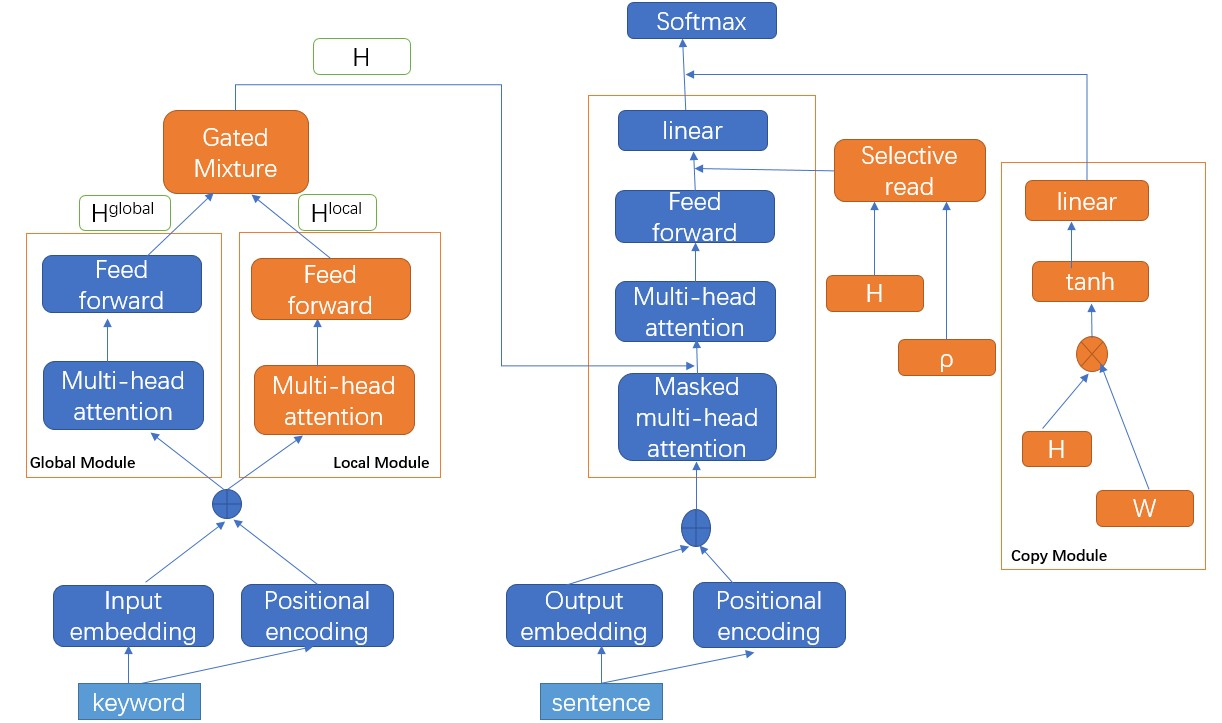
\includegraphics[width=12cm,height=8cm]{model2.jpg}
\caption{Global-Local-Copy Model}\label{fig:model}
\end{figure*}

\begin{equation}\label{equ:mixture}
    \mathbf{H} = \beta^s\mathbf{H}^{local} + (1-\beta^s)\mathbf{H}^{global}.
\end{equation}
Here, the scalar $\beta$ is a learned parameter between 0 and 1 that is specific to the scenario $s$.

\textbf{Decoder:} The copy module is in decoder module, the probability of generating any target word $y_t$, is given by the mixture of probabilities as follows

\begin{equation}\label{equ:mixture-prob}
    p(y_t) = p(y_t,g) + p(y_t,c)
\end{equation}

where $g$ stands for the generate-mode, and $c$ the
copy mode. the right of Fig.~\ref{fig:model} illustrates the copy module decoder. $H$ is global-local encoding the above-mentioned, $\zeta(y)$ is the weighted sum of hidden states $H$ corresponding to $y$, referred to as selective read in the right of Fig.~\ref{fig:model}. 

\begin{equation}\label{equ:zeta}
    \zeta(y) = \sum^{T}_{\tau = 1} \rho_\tau \textbf{h}_\tau 
\end{equation}

\begin{equation}\label{equ:rho}
    \rho_\tau = \left\{
        \begin{aligned}
        \frac{1}{K} p(x_\tau,\textbf{c}|\textbf{H}), \quad & x_\tau = y_t & \\
        0, \quad & otherwise &
        \end{aligned} 
        \right.
\end{equation}

where $K$ is equal to the number of positions with source keywords in the target sentence, $\tau$ is the index of source keywords, $T$ is the number of keywords, $t$ is the index of word in target sentence, and $p(x_\tau,\textbf{c}|\textbf{H})$ is the probability of the source keyword be copied in target sentence. 

The score of each mode is calculated:

\textbf{Generate-Mode}: first connect the output of the feed forward part of the transformer method and selective-read, and then $p(y_t,g)$ is calculated through the full connection. 

\textbf{Copy-Mode}: first calculate $\sigma(\textbf{H}\textbf{W})$, $\sigma$ is a non-linear activation function, here using the $tanh$ function. Next $p(y_t,c)$ is calculated through the full connection. 

\section{EXPERIMENTAL SETUP}\label{sec:experiment}
\subsection{Dataset}
In this paper,we focus on two sub-scenarios under the home: creative home and simple home. We select the description of the products in these two scenarios from the list of product recommendation reasons. We collected 150,743 sentences related to these products, after weak supervision, left 103,612 sentences. We chose sentences which keyword input only appears once as the test set. Training data format is shown in Tab.~\ref{table:format}. 

\begin{table}
\caption{Training data format }\label{table:format}
\begin{center}
\begin{tabular}{p{2.5cm}p{5cm}}
    \toprule
    Input & Output \\
    \midrule
    \begin{CJK*}{UTF8}{gbsn}
        创意,纸巾盒,欧式
    \end{CJK*} &
    \begin{CJK*}{UTF8}{gbsn}
        一款欧式风范榉木纸巾盒,盒身采用创意撞色设计,不仅能放杂物,还能作为桌面摆设,大中小三种尺寸可选,适合多种场合使用。
    \end{CJK*} \\
    \bottomrule
\end{tabular}
\end{center}
\end{table}

\subsection{Comparative Method}
%WWW这篇有一步寻找名词短语,我的替换方法是 形容词(1个或多个)+ 的 + 名词(0个或1个) 例如: 浪漫的荷花  这样子的词语
%None Phrase Selection部分,改成寻找【形容词(1个或多个)+ ‘的’ + 名词(0个或1个)】的短语,因为文中没有提到KeywordExpansion部分的k和None Phrase Selection部分的L取值,我就选了k=5和l=10,其他都和文中一样

\subsection{Training}
We take the words from source side of corpus as the input vocabulary and chose the words from target side of corpus which word frequency greater than 20 as the output vocabulary. The dimension of word embedding and hidden units are both 512,the minibatch was set to be 64. The parameter of global-local module $\beta$ is initialized by 0.5, the parameter $W$ in copy module is randomly initialized and the the parameter $p$ is initialized by zero.

\subsection{Evaluation}
There are no direct evaluation metrics so that evaluate text generation system is difficult.  We choose ROUGE \cite{lin2004rouge} and BLEU \cite{papineni2002bleu} metrics that are popularly used for generation tasks (especially Machine Translation and Summarization). These two metrics are both based on references, but there are thousands of ways to generate an appropriate sentence for a specific product,the limited references are impossible to cover all the correct results. So,we we use five evaluation standards for human evaluators to check the quality of the generated descriptions on a small test dataset of 30 instances. The manual evaluation metrics are listed in Tab.~\ref{table:evaluation}. The score of each manual evaluation metrics ranges from 0 to 5 with the higher score the better, see Tab.~\ref{table:evaluation-rule} for more detailed Grading Rules. All the generated sentences are evaluated by 5 experts and the rating scores are averaged as the final score.

\begin{table}
\caption{Manual Evaluation }\label{table:evaluation}
\begin{center}
\begin{tabular}{p{2.5cm}p{5cm}}
    \toprule
    Evaluation Metric & Description \\
    \midrule
    Fluency \cite{wang2016chinese} & Does the sentence read smoothly and fluently? \\
    Catchyness \cite{munigala2018persuaide} & Is the description attractive,catchy? \\
    Relatedness \cite{munigala2018persuaide} & Is the description semantically related to the target scene? \\
    Completeness & Is the description contains the corresponding scene, product and attribute? \\
    Informative & Is the description informative?\\
    \bottomrule
\end{tabular}
\end{center}
\end{table} 

\begin{table}
\caption{Manual Evaluation details}\label{table:evaluation-rule}
\begin{center}
\begin{tabular}{p{2.5cm}p{1cm}p{4.5cm}}
    \toprule
    Evaluation Metric & Score & Description \\
    \midrule
    \multirow{3}*{Fluency} & 0 & Not at all smooth \\
    ~ & 1-4 & how many places are not smooth minus how many points \\
    ~ & 5 & Very smooth\\
    \hline
    Catchyness & 0-5 & The ratio of attractive words in total words multiply by 5\\
    \hline
    \multirow{4}*{Relatedness} & 0 & Completely unrelated to the scene \\
    ~ & 1 & none \\
    ~ & 2 & Refer to the scene \\ 
    ~ & 3-5 & how many descriptions related to the scene, add how many points\\
    \hline
    \multirow{6}*{Completeness} & 0 & No input at all \\
    ~ & 1 & none \\
    ~ & 2 & Contains an input keyword \\ 
    ~ & 3 & Contains two input keyword\\
    ~ & 4 & There's no third word involved, but it's relevant\\
    ~ & 5 & Completely contains\\
    \hline
    \multirow{3}*{Informative} & 0 & No information at all \\
    ~ & 1 & It's describing the product \\
    ~ & 2-5 & how much information about the product, add how many points\\
    \bottomrule
\end{tabular}
\end{center}
\end{table} 

\subsection{Results}
We report the experimental results for our two approaches, i.e. global-local model and global-local-copy model. The difference between two models is former has no copy module. We compare our models with the Transformer method. Results are reported on the test data of 1472 instances, used for automatic evaluation and a held-out set of 32 instances, used for manual evaluation. The source keyword of test data for automatic evaluation are never appeared in train data. We choose the source keyword of test data that have scene name, product name and only one cpv value for manual evaluation.

From the perspective of considering our system as another machine translation system that converts some keywords of product(the scene name, product name, cpv data) into a persuasive product description with scene, we have results shown in Tab.~\ref{table:evaluation-automatic}. Popular machine translation and summarization metrics BLEU and ROUGE are used. There are four different ROUGE measures: ROUGE-N, ROUGE-L, ROUGE-W, and ROUGE-S, depending on the textual units to be compared. As can be seen from the results, our two methods are superior to Transformer in every indicator. Explain that both the global-local module and the copy module have a positive impact on the model. Because these two metrics are both based on references, and the copy module is aim to let the output sentence contain user-supplied input, so the results of global-local-copy model is better than global-local model.

\begin{table}
  \caption{Automatic Evaluation Metrics}
  \label{table:evaluation-automatic}
  \begin{tabular}{c c c c}
    \toprule
    Metrics & Transformer & Global-local & Global-local-copy\\
    \midrule
    ROUGE-1 & 0.3933 & 0.4050 & 0.4054\\
    ROUGE-2 & 0.1319 & 0.1446 & 0.1488\\
    ROUGE-3 & 0.0643 & 0.0740 & 0.0777\\
    ROUGE-4 & 0.0424 & 0.0514 & 0.0521\\
    ROUGE-L & 0.3259 & 0.3373 & 0.3423\\
    ROUGE-W & 0.1491 & 0.1552 & 0.1585\\
    ROUGE-S* & 0.1628 & 0.1762 & 0.1784\\
    BLEU-1 & 0.2964 & 0.3056 & 0.3096\\
    BLEU-2 & 0.1556 & 0.1671 & 0.1729\\
    BLEU-3 & 0.0807 & 0.0926 & 0.0977\\
    BLEU-4 & 0.0522 & 0.0632 & 0.0654\\
  \bottomrule
\end{tabular}
\end{table}

From the perspective of human psychology of persuasive product descriptions, we manually evaluated the generated descriptions using human evaluators. Five different measures were used to evaluate the human subjectiveness: Catchyness, Relatedness, Fluency, Completeness and Informative. It can be evidently observed in Tab.~\ref{table:evaluation-manual}. that the proposed system generated more catchy, better related, more fluency sentences compared to the Transformer method. Because our global-local module focuses on the description of the scene, resulting in the generated sentences with more descriptions of the scene, more appealing and more relevant to the scene. What's more, sentences generated by our model contain more input keywords and have more information about product.

\begin{table}
  \caption{Manual Evaluation Metrics}
  \label{table:evaluation-manual}
  \begin{tabular}{c c c c}
    \toprule
    Metrics & Transformer & Global-local & Global-local-copy\\
    \midrule
    Catchyness & 1.2235 & 1.2455 & 1.3320\\
    Relatedness & 2.4375 & 2.5000 & 2.7500\\
    Fluency & 3.4375 & 3.7187 & 3.9375\\
    Completeness & 3.6250 & 3.9375 & 3.9062\\
    Informative & 3.0312 & 3.4687 & 3.4687 \\
  \bottomrule
\end{tabular}
\end{table}

For qualitative analysis, we also provide the sentences generated from our system as well as other systems in the Tab.~\ref{table:case}. As we can see, the descriptions generated by our systems are competitive or better in terms of creativity, persuasiveness and fluency than the supervised baselines but have less overlap with the reference descriptions. This explains why our system is deemed to have underperformed than the baselines, as per the automatic evaluation scores. In general, the field of creative text generation demands looking beyond simplistic evaluation measures and it is about time that trainable metrics for evaluating persuasive text holistically, including aspects on creativity, coherency, novelty are proposed.

\begin{table*}
  \caption{Sample generations from different systems along with inputs and reference descriptions}
  \label{table:case}
  \begin{tabular}{p{2.5cm}p{12cm}}
    \hline
    Input & 
    \begin{CJK*}{UTF8}{gbsn}
        创意,挂钟,奢华
    \end{CJK*} \\
    Transformer & 
    \begin{CJK*}{UTF8}{gbsn}
        创意 十足 的 挂钟 , 舒适 静音 的 设计 , 温柔 的 花纹 , 灵动 而 神秘 , 让 你 爱 坐在 客厅 的 时光 里 里 静静 享受 质量 。
    \end{CJK*} \\
    Global-local & 
    \begin{CJK*}{UTF8}{gbsn}
        创意 挂钟 , 奢华 镶 钻 , 奢华 镶 钻 , 奢华 镶 钻 。
    \end{CJK*} \\
    Global-local-copy & 
    \begin{CJK*}{UTF8}{gbsn}
        创意 十足 的 大 号 挂钟 , 奢华 范 , 奢华 独特 。
    \end{CJK*} \\
    \hline
    Input & 
    \begin{CJK*}{UTF8}{gbsn}
        简约,挂钟,精致
    \end{CJK*} \\
    Transformer & 
    \begin{CJK*}{UTF8}{gbsn}
        简约 静音 挂钟 , 做工 精致 , 细节 精致 , 高档 品质 之选 。
    \end{CJK*} \\
    Global-local & 
    \begin{CJK*}{UTF8}{gbsn}
        可 摇摆 的 静音 挂钟 , 做工 精致 , 造型 独特 , 简约 大气 的 外形 符合 你 的 工作 品质 生活 , 静音 设计 , 增加 家中 的 灵动 性 。
    \end{CJK*} \\
    Global-local-copy & 
    \begin{CJK*}{UTF8}{gbsn}
        这 款 挂钟 , 造型 简约 大方 , 做工 精致 , 散发 着 大自然 的 气息 , 选用 的 静音 扫描 机芯 , 走时 准确 , 可 挂 在 墙上 , 方便 又 不 掉色 。
    \end{CJK*} \\
  \bottomrule
\end{tabular}
\end{table*}

\section{Conclusion}\label{sec:conclusion}

\section{Acknowledgments}

\bibliographystyle{ACM-Reference-Format}
\bibliography{refer.bib}
\end{document}
